\documentclass{article}
\linespread{1.3}
\usepackage[margin=50pt]{geometry}
\usepackage{amsmath, amsthm, amssymb, amsthm,fancyhdr, graphicx, tikz}
\pagestyle{fancy}
\renewcommand{\headrulewidth}{0pt}
\newcommand{\changefont}{\fontsize{15}{15}\selectfont}

\newcommand{\field}[1]{\mathbb{#1}}
\newcommand{\1}{\mathbf{1}}
\newcommand{\E}{\mathbb{E}} 
\renewcommand{\P}{\mathbb{P}}
\newcommand{\R}{\field{R}} % real domain
% \newcommand{\C}{\field{C}} % complex domain
\newcommand{\F}{\field{F}} % functional domain

\newcommand{\T}{^{\textrm T}} % transpose

\def\diag{\text{diag}}

%% operator in linear algebra, functional analysis
\newcommand{\inner}[2]{#1\cdot #2}
\newcommand{\norm}[1]{\left\|#1\right\|}
\newcommand{\twonorm}[1]{\|#1\|_2^2}
% operator in functios, maps such as M: domain1 --> domain 2
\newcommand{\Map}[1]{\mathcal{#1}}
\renewcommand{\theenumi}{\alph{enumi}} 

\newcommand{\Perp}{\perp \! \! \! \perp}

\newcommand\independent{\protect\mathpalette{\protect\independenT}{\perp}}
\def\independenT#1#2{\mathrel{\rlap{$#1#2$}\mkern2mu{#1#2}}}
\newcommand{\vct}[1]{\boldsymbol{#1}} % vector
\newcommand{\mat}[1]{\boldsymbol{#1}} % matrix
\newcommand{\cst}[1]{\mathsf{#1}} % constant
\newcommand{\ProbOpr}[1]{\mathbb{#1}}
\newcommand{\points}[1]{\small\textcolor{magenta}{\emph{[#1 points]}} \normalsize}
\date{{}}

\fancypagestyle{firstpageheader}
{
  \fancyhead[R]{\changefont Michael Huang \\ CSE 446 \\ Homework 0}
}

\begin{document}

\thispagestyle{firstpageheader}

\section*{A.1}
{\Large 

Bayes' Rule tells us that $P(A \mid B) = \frac{P(A \cap B)}{P(B)} = \frac{P(B \mid A) \cdot P(A)}{P(B)}$. Let $A$ = the event that we have the disease, and $B$ = the event that we test positive for the disease. We aim to find the probability that we have the disease, given that we tested positive, i.e. $P(A \mid B)$. We are given that $P(A) = \frac{1}{10,000}$, $P(B \mid A) = \frac{99}{100}$. \\ \\ 
We need to find $P(B)$, the probability that we test positive for the disease. To do this, we can use the Law of Total Probability to add up the probabilities for its contained disjoint events $A$ and $\lnot A$: \\
$P(B) = P(B | A)P(A) + P(B | \lnot A)P(\lnot A)$ \\ 
$P(B) = \frac{99}{100} \cdot \frac{1}{10,000} + \frac{1}{100} \cdot (1 - \frac{1}{10,000})$ \\
$P(B) = \frac{99}{100} \cdot \frac{1}{10,000} + \frac{1}{100} \cdot \frac{9,999}{10,000}$ \\
$P(B) = \frac{99}{1,000,000} + \frac{9,999}{1,000,000}$ \\
$P(B) = \frac{10,098}{1,000,000}$ \\ \\
Putting this all together, we can find that \\
$P(A \mid B) = \frac{P(B \mid A) \cdot P(A)}{P(B)} = \frac{\frac{99}{100} \cdot \frac{1}{10,000}}{\frac{10,098}{1,000,000}} = \frac{99}{10,098} = $ \framebox[1.1\width]{\textbf{$\frac{1}{102}$ or $\sim 0.00980392156863$}} \\ 


}

\section*{A.2}
{\Large

\subsection*{a.}
We know that by the definition of covariance: \\
$\text{Cov}(X,Y)=\E[(X-\E[X])(Y-\E[Y])]$ \\
$\text{Cov}(X,Y)=\E[XY - \E[X]Y - \E[Y]X + \E[X]\E[Y]]$ \\
$\text{Cov}(X,Y)=\E[XY] - \E[X]\E[Y] - \E[Y]\E[X] + \E[X]\E[Y]$ \\
$\text{Cov}(X,Y)=\E[XY] - \E[Y]\E[X]$ \\ \\
We are given that $\E[Y \mid X=x ] = x$. This tells us that for any value $X = x$, $E[Y] = x$ as well. We know by definition that $\E[X] = \sum_{x} x \cdot \P(X = x)$. We also know that $\E[Y] = \sum_{x} \E[Y \mid X = x] \cdot \P(X = x)$. \\
Using what we are given, we can easily see that $\E[Y] = \sum_{x} x \cdot \P(X = x) = \E[X]$, or that $\E[X] = \E[Y]$. \\
% TODO: Explanation
In the same vein, in our case, using the given information to represent $Y = y$ in terms of $X$, we can determine that $\E[XY] = \sum_x x \cdot y \cdot \P(X = x) = \sum_x x \cdot x \cdot \P(X = x) = \E[X^2]$. In other words, $\E[XY] = \E[X^2]$.\\ \\
Using this information, we can simplify this expression to \\
$\text{Cov}(X,Y)= \E[XY] - \E[X]\E[X]$ \\
$\text{Cov}(X,Y)= \E[X^2] - \E[X]^2$ \\
$\text{Cov}(X,Y)= \text{Var}(X)$ \\
$\text{Cov}(X,Y)= \E[(X - \E[X])^2]$ \\
as desired.

\subsection*{b.}
Since $X, Y$ are independent, then $\E[XY] = \E[X]\E[Y]$. Using the expression that we derived in part a, we can determine that $\text{Cov}(X,Y)=\E[XY] - \E[Y]\E[X] = \E[X]\E[Y] - \E[Y]\E[X] = \E[X]\E[Y] - \E[X]\E[Y] = 0$, as desired.

}

\section*{A.3}
{\Large 

\subsection*{a.}
% TODO: Leibnetz Rule?
We aim to find the PDF $h$ of the random variable $Z = X + Y$, where $X$ and $Y$ are independent random variables with PDFs given by $f$ and $g$, respectively. In addition, let $H$, $F$, and $G$ represent the CDFs of $Z$, $X$, and $Y$, respectively. \\ \\
By definition of CDF, we can take \\ 
$H(z) = \P(Z \leq z) = \P(X + Y \leq z)$. \\
$H(z) = \int_{-\infty}^{\infty} \int_{-\infty}^{z-x} f(x) g(y) \,dy \,dx$ \hfill Independence of $X$ and $Y$ \\ 
$H(z) = \int_{-\infty}^{\infty} f(x) G(z - x) \,dx$ \hfill Definition of CDF \\ 
$\frac{d}{dz} H(z) = \frac{d}{dz} \int_{-\infty}^{\infty} f(x) G(z - x) \,dx$ \hfill Definition of PDF \\ 
$h(z) = \int_{-\infty}^{\infty} f(x) \cdot \frac{d}{dz} G(z - x) \,dx$ \hfill Definition of PDF \\ 
$h(z) = \int_{-\infty}^{\infty} f(x) g(z - x) \,dx$ \hfill Derivatives \\ 
$h(z) = \int_{-\infty}^{\infty} g(z-x) f(x) \,dx$ \hfill Algebra \\
as we sought to show.

\subsection*{b.}
We aim to find $h(z)$. Using what we showed in part a, \\
$h(z) = \int_{-\infty}^{\infty} g(z - x) f(x) \,dx$ \\ 
$h(z) = \int_{0}^{1} g(z-x) \,dx$ \hfill Definition of Uniform Distribution of $X$ \\ \\
We can break this expression into two different cases: where $z = x + y \leq 1$ or not, which we must do since we know that $x$ and $y$ are restricted in the range $[0, 1]$: \\
Case 1: $0 \leq z \leq 1$ \\ 
$h(z) = \int_{0}^{z} g(z-x) \,dx + \int_{z}^{1} g(z-x) \,dx$ \\ 
$h(z) = z \cdot 1 + 0 = z$ \\
Case 2: $1 < z \leq 2$ \\ 
$h(z) = \int_{0}^{z-1} g(z-x) \,dx + \int_{z-1}^{1} g(z-x) \,dx$ \\ 
$h(z) = 1 + 1 - z = 2-z$ \\ \\
Putting this all together, the PDF $h$ is as follows:
\[
h\left(z\right)=\begin{cases}
z & \,0\le z\le1;\\
2 - z & \,1< z\le2;\\
0 & \,\mbox{otherwise,}\\
\end{cases}
\]

}

\section*{A.4}
{\Large 

We aim to find $a, b$ such that $Y = aX + b$. We know that the standard normal is defined by $Y = \frac{X - \mu}{\sigma} = \frac{X}{\sigma} - \frac{\mu}{\sigma} = \frac{1}{\sigma}X - \frac{\mu}{\sigma}$. In the $aX + b$ form, we can see that this translates to \framebox[1.1\width]{\textbf{$a = \frac{1}{\sigma}$ and $b = -\frac{\mu}{\sigma}$}}

}

\section*{A.5}
{\Large 
We aim to find the mean and variance of $Z = \sqrt{n}(\widehat{\mu}_n - \mu)$, where $\widehat{\mu}_n = \frac{1}{n} \sum_{i=1}^n X_i$, and $X_1,\dots,X_n$ are independent and identically distributed random variables, each with mean $\mu$ and variance $\sigma^2$. \\ \\
To find the mean: \\
$\E[Z] = \E[\sqrt{n}(\widehat{\mu}_n - \mu)]$ \\
$\E[Z] = \sqrt{n}\E[\widehat{\mu}_n - \mu]$ \\
$\E[Z] = \sqrt{n}\E[\widehat{\mu}_n] - \E[\mu]$ \\
$\E[Z] = \sqrt{n}(\mu - \mu)$ \hfill Given \\
$\E[Z] = $ \framebox[1.1\width]{\textbf{0}} \\ \\
To find the variance: \\
$\text{Var}(Z) = \E[Z^2] - \E[Z]^2$ \\
$\text{Var}(Z) = \E[Z^2] - 0^2$ \\
$\text{Var}(Z) = \E[Z^2]$ \\
$\text{Var}(Z) = \E[(\sqrt{n}(\widehat{\mu}_n - \mu))^2]$ \\
$\text{Var}(Z) = \E[n \cdot (\widehat{\mu}_n - \mu)^2]$ \\
$\text{Var}(Z) = \E[n \cdot (\widehat{\mu}_n^2 + \mu^2 - 2\widehat{\mu}_n \mu)]$ \\
$\text{Var}(Z) = n \cdot \E[\widehat{\mu}_n^2 + \mu^2 - 2\widehat{\mu}_n \mu]$ \\
$\text{Var}(Z) = n \cdot (\E[\widehat{\mu}_n^2] + \E[\mu^2] - \E[2\widehat{\mu}_n \mu])$ \\
$\text{Var}(Z) = n \cdot (\E[\widehat{\mu}_n^2] - \E[\widehat{\mu}_n]^2 + \E[\widehat{\mu}_n]^2 + \mu^2 - 2\mu\E[\widehat{\mu}_n])$ \\
$\text{Var}(Z) = n \cdot (\text{Var}(\widehat{\mu}_n) + \E[\widehat{\mu}_n]^2 + \mu^2 - 2\mu\E[\widehat{\mu}_n])$ \\
$\text{Var}(Z) = n \cdot (\frac{\sigma^2}{n} + \mu^2 + \mu^2 - 2\mu^2)$ \hfill Given \\
$\text{Var}(Z) = $ \framebox[1.1\width]{\textbf{$\sigma^2$}}

}

\section*{A.6}
{\Large 

We are given that the empirical estimate of $F(x)$ as $\widehat{F}_n(x) = \frac{1}{n} \sum_{i=1}^n \1\{X_i \leq x\}$.

\subsection*{a.}
We aim to find $\E[ \widehat{F}_n(x) ]$ for any $x$: \\
$\E[ \widehat{F}_n(x) ] = \E[\frac{1}{n} \sum_{i=1}^n \1\{X_i \leq x\}] = \frac{1}{n} \sum_{i=1}^n \E[\1\{X_i \leq x\}] = \frac{1}{n} \sum_{i=1}^n \1\{X_i \leq x\} = $ \framebox[1.1\width]{\textbf{$F(x)$}}

\subsection*{b.}
We aim to show that $\textrm{Var}(\widehat{F}_n(x)) = \frac{F(x)(1-F(x))}{n}$. We know that the variance of a Bernoulli random variable as we defined is $\text{Var}(X) = p(1-p)$, which tells us that $\text{Var}(F(x)) = F(x)(1-F(x))$ in our case. Using our previous definitions, we know that \\
$\textrm{Var}(\widehat{F}_n(x)) = \frac{1}{n^2} \sum_{i = 1}^{n} Var(X_i)$ \\
$\textrm{Var}(\widehat{F}_n(x)) = \frac{1}{n^2} \cdot \sum_{i = 1}^{n} F(x)(1-F(x))$ \\ 
$\textrm{Var}(\widehat{F}_n(x)) = \frac{1}{n} \cdot F(x)(1-F(x))$ \\ 
$\textrm{Var}(\widehat{F}_n(x)) = \frac{F(x)(1-F(x))}{n}$ \\
as we sought to show.

\subsection*{c.}
We aim to show that for all $x \in \R$, we have  $\displaystyle \E[ ( \widehat{F}_n(x) - F(x) )^2 ] \leq \tfrac{1}{4n}$. By definition and using what we showed previously, we know that $\displaystyle \E[ ( \widehat{F}_n(x) - F(x) )^2 ] = \text{Var}(\widehat{F}_n(x)) = $ $\frac{F(x)(1-F(x))}{n}$. Since we aim to limit the variance to $\frac{1}{4n}$, we can find the determine the critical point by taking the derivative: \\ \\ 
$\frac{d}{dx} F(x)(1 - F(x)) = 0$ \\
$\frac{d}{dx} F(x) \cdot (1 - F(x)) + F(x) \cdot \frac{d}{dx} (1 - F(x)) = 0$ \\
$f(x) \cdot (1 - F(x)) + F(x) \cdot -f(x) = 0$ \\
$f(x) - f(x)F(x)) - F(x)f(x) = 0$ \\
$f(x) - 2 f(x)F(x)) = 0$ \\ \\
We see that $F(x) = \frac{1}{2}$, which is its maximum. Plugging this into our original equation: \\
$\displaystyle \E[ ( \widehat{F}_n(x) - F(x) )^2 ] = \text{Var}(\widehat{F}_n(x)) = $ $\frac{\frac{1}{2}(1-\frac{1}{2})}{n}$ \\ 
$\displaystyle \E[ ( \widehat{F}_n(x) - F(x) )^2 ] = \text{Var}(\widehat{F}_n(x)) = $ $\frac{\frac{1}{4}}{n}$ \\ 
$\displaystyle \E[ ( \widehat{F}_n(x) - F(x) )^2 ] = \text{Var}(\widehat{F}_n(x)) = $ $\frac{1}{4n}$ \\
which is the maximum value of the variance according to our critical point. We have therefore shown that $\displaystyle \E[ ( \widehat{F}_n(x) - F(x) )^2 ] \leq \tfrac{1}{4n}$.

}

\section*{A.7}
{\Large 

\subsection*{a.}
To find rank, we use row reduction and find how many unique non-zero rows are left once we reach row echelon form: \\ \\
$A = \begin{bmatrix} 1 & 2 & 1 \\ 1 & 0 & 3 \\ 1 & 1 & 2 \end{bmatrix}$ 
$ = \begin{bmatrix} 1 & 2 & 1 \\ 0 & -2 & 2 \\ 0 & -1 & 1 \end{bmatrix}$
$ = \begin{bmatrix} 1 & 2 & 1 \\ 0 & -2 & 2 \\ 0 & 0 & 0 \end{bmatrix}$ \\
With only 2 unique non-zero rows left, we can see that \framebox[1.1\width]{\textbf{the rank of $A$ is 2}} \\ \\
$B = \begin{bmatrix} 1 & 2 & 3 \\ 1 & 0 & 1 \\ 1 & 1 & 2 \end{bmatrix}$ 
$ = \begin{bmatrix} 1 & 2 & 3 \\ 0 & -2 & -2 \\ 0 & -1 & -1 \end{bmatrix}$
$ = \begin{bmatrix} 1 & 2 & 3 \\ 0 & -2 & -2 \\ 0 & 0 & 0 \end{bmatrix}$ \\ 
With only 2 unique non-zero rows left, we can see that \framebox[1.1\width]{\textbf{the rank of $B$ is 2}}

\subsection*{b.}
To find the minimal size basis for the column span of a matrix, we need to look at the pivot columns of the row echelon form matrix and then take those columns to get the basis:
$A = \begin{bmatrix} 1 & 2 & 1 \\ 1 & 0 & 3 \\ 1 & 1 & 2 \end{bmatrix}$ 
$ = \begin{bmatrix} 1 & 2 & 1 \\ 0 & -2 & 2 \\ 0 & -1 & 1 \end{bmatrix}$
$ = \begin{bmatrix} 1 & 2 & 1 \\ 0 & -2 & 2 \\ 0 & 0 & 0 \end{bmatrix}$ \\
Taking the first 2 columns, we get \\
$ = \begin{bmatrix} 1 & 2 \\ 1 & 0 \\ 1 & 1 \end{bmatrix}$ \\ \\
$B = \begin{bmatrix} 1 & 2 & 3 \\ 1 & 0 & 1 \\ 1 & 1 & 2 \end{bmatrix}$ 
$ = \begin{bmatrix} 1 & 2 & 3 \\ 0 & -2 & -2 \\ 0 & -1 & -1 \end{bmatrix}$
$ = \begin{bmatrix} 1 & 2 & 3 \\ 0 & -2 & -2 \\ 0 & 0 & 0 \end{bmatrix}$ \\ 
Taking the first 2 columns, we get \\
$ = \begin{bmatrix} 1 & 2 \\ 1 & 0 \\ 1 & 1 \end{bmatrix}$

}

\section*{A.8}
{\Large 

Let $A = \begin{bmatrix} 0 & 2 & 4 \\ 2 & 4 & 2 \\ 3 & 3 & 1 \end{bmatrix}$, $b = \begin{bmatrix} -2 & -2 & -4 \end{bmatrix}^T$, and $c=\begin{bmatrix} 1 & 1 & 1 \end{bmatrix}^T$.

\subsection*{a.}
$Ac = \begin{bmatrix} 0 & 2 & 4 \\ 2 & 4 & 2 \\ 3 & 3 & 1 \end{bmatrix} \cdot \begin{bmatrix} 1 & 1 & 1 \end{bmatrix}^T$ \\ 
$= \begin{bmatrix} 0 & 2 & 4 \\ 2 & 4 & 2 \\ 3 & 3 & 1 \end{bmatrix} \cdot \begin{bmatrix} 1 \\ 1 \\ 1 \\ \end{bmatrix}$ \\
$= \begin{bmatrix} 0 \cdot 1 + 2 \cdot 1 + 4 \cdot 1 \\ 2 \cdot 1 + 4 \cdot 1 + 2 \cdot 1 \\ 3 \cdot 1 + 3 \cdot 1 + 1 \cdot 1 \end{bmatrix}$ \\
$= \begin{bmatrix} 6 \\ 8 \\ 7 \end{bmatrix}$

\subsection*{b.}
$Ax = b$ \\
$\begin{bmatrix} 0 & 2 & 4 \\ 2 & 4 & 2 \\ 3 & 3 & 1 \end{bmatrix} x = \begin{bmatrix} -2 & -2 & -4 \end{bmatrix}^T$ \\ 
$\begin{bmatrix} 0 & 2 & 4 \\ 2 & 4 & 2 \\ 3 & 3 & 1 \end{bmatrix} x = \begin{bmatrix} -2 \\ -2 \\ -4 \end{bmatrix}$ \\ 
$\left[
\begin{array}{ccc|c}
0 & 2 & 4 & -2 \\
2 & 4 & 2 & -2 \\
3 & 3 & 1 & -4 \\
\end{array}
\right]$ =
$\left[
\begin{array}{ccc|c}
2 & 4 & 2 & -2 \\
0 & 2 & 4 & -2 \\
3 & 3 & 1 & -4 \\
\end{array}
\right]$ =
$\left[
\begin{array}{ccc|c}
1 & 2 & 1 & -1 \\
0 & 1 & 2 & -1 \\
3 & 3 & 1 & -4 \\
\end{array}
\right]$ =
$\left[
\begin{array}{ccc|c}
1 & 2 & 1 & -1 \\
0 & 1 & 2 & -1 \\
0 & -3 & -2 & -1 \\
\end{array}
\right]$ =
$\left[
\begin{array}{ccc|c}
1 & 2 & 1 & -1 \\
0 & 1 & 2 & -1 \\
0 & 0 & 4 & -4 \\
\end{array}
\right]$ =
$\left[
\begin{array}{ccc|c}
1 & 2 & 1 & -1 \\
0 & 1 & 2 & -1 \\
0 & 0 & 1 & -1 \\
\end{array}
\right]$ =
$\left[
\begin{array}{ccc|c}
1 & 2 & 1 & -1 \\
0 & 1 & 0 & 1 \\
0 & 0 & 1 & -1 \\
\end{array}
\right]$ =
$\left[
\begin{array}{ccc|c}
1 & 2 & 0 & 0 \\
0 & 1 & 0 & 1 \\
0 & 0 & 1 & -1 \\
\end{array}
\right]$ =
$\left[
\begin{array}{ccc|c}
1 & 0 & 0 & -2 \\
0 & 1 & 0 & 1 \\
0 & 0 & 1 & -1 \\
\end{array}
\right]$ \\ \\
So our result is therefore \\ \\
$\begin{bmatrix} -2 \\ 1 \\ -1 \end{bmatrix}$ 

}

\section*{A.9}
{\Large 

Assume $w$ is an $n$-dimensional vector and $b$ is a scalar. A hyperplane in $\R^n$ is the set $\{x : x\in \R^n,\text{ s.t. } w^T x + b = 0\}$.

\begin{verbatim}
def get_zvalue(x, y):
  return -x - y

def plot_hyperplanes():
  print("A.9.a")

  x = np.arange(-100, 100)
  y = np.arange(-100, 100)
  plt.title("A.9.a")
  plt.xlabel("x-values")
  plt.ylabel("y-values")
  plt.xlim(-10, 10)
  plt.ylim(-10, 10)
  plt.plot(x, 0 * x)
  plt.plot(0 * y, y)
  plt.plot(x, 0.5 * x - 1)
  plt.savefig("A9a.png")
  plt.close()

  print("A.9.b")
  fig = plt.figure()
  ax = plt.axes(projection='3d')

  # x and y axis
  x = np.linspace(-80, 80)
  y = np.linspace(-80, 80)
  z = np.linspace(-80, 80)

  xo = np.linspace(-100, 100)
  yo = np.linspace(-100, 100)
  zo = np.linspace(-100, 100)
  
  X, Y = np.meshgrid(x, y)
  Z = get_zvalue(X, Y)
  
  ax.plot_surface(X, Y, Z, rstride=1, cstride=1,
                cmap='viridis', edgecolor='none')
  ax.plot3D(xo, yo * 0, zo * 0)
  ax.plot3D(xo * 0, yo, zo * 0)
  ax.plot3D(xo * 0, yo * 0, zo)
  ax.set_title("A.9.b")
  
  ax.set_xlabel("x-values")
  ax.set_ylabel("y-values")
  ax.set_zlabel("z-values")
  
  plt.savefig("A9b.png");
  plt.close()
\end{verbatim}

\subsection*{a.}
We substitute for $w^T x + b = 0$ and plot: \\
$w = \begin{bmatrix} -1 & 2 \\ \end{bmatrix}$ \\
$w^T = \begin{bmatrix} -1 \\ 2 \\ \end{bmatrix}$ \\
$\begin{bmatrix} -1 \\ 2 \\ \end{bmatrix}$ x = -2 \\
$-x + 2y = -2$ \\
$y = \frac{1}{2}x -1$ \\ \\ \\ \\ \\ \\

\begin{figure}[ht!]
  \centering
  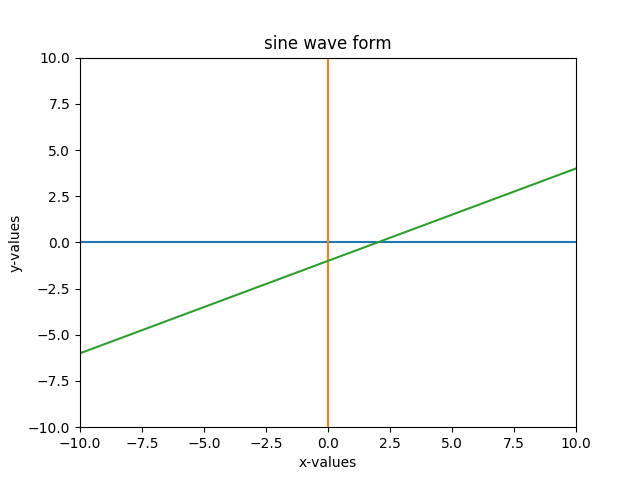
\includegraphics[width=150mm]{A9a.PNG}
\end{figure}

\subsection*{b.}
We solve for $w^T x + b = 0$: \\
$w = \begin{bmatrix} 1 & 1 & 1 \\ \end{bmatrix}$ \\
$w^T = \begin{bmatrix} 1 \\ 1 \\ 1 \\ \end{bmatrix}$ \\
$\begin{bmatrix} 1 \\ 1 \\ 1 \\ \end{bmatrix} x = 0$ \\ 
$x + y + z = 0$ \\
$z = -x - y$ \\

\begin{figure}[ht!]
  \centering
  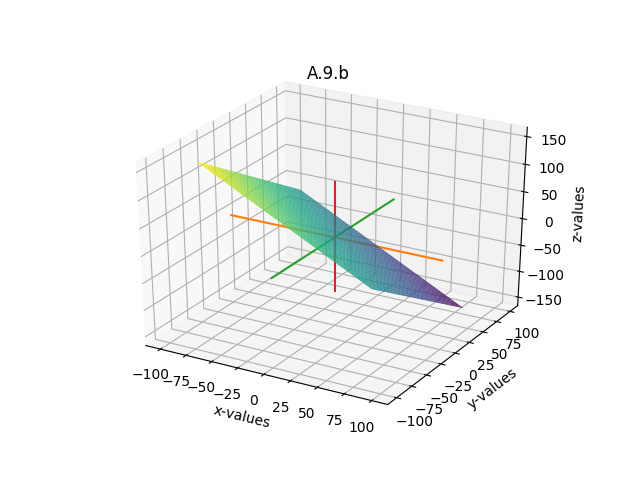
\includegraphics[width=180mm]{A9b.PNG}
\end{figure}

\subsection*{c.}
We are given some arbitrary point $x_0 \in \R^n$ and some hyperplane defined by $w^Tx + b = 0$, as well as some point on the hyperplane $ \widetilde{x}_0$. \\ \\
We can measure the minimal distance from the arbitrary point to the closest point on the hyperplane using an orthogonal projection. We can calculate this using dot products as follows: \\
$\| \text{proj}_{x_0, \widetilde{x}_0} \| = \| \frac{(x_0 - \widetilde{x}_0) \cdot w^T}{w^T \cdot w^T} \cdot w^T \| = |(x_0 - \widetilde{x}_0) \cdot w^T| \cdot \frac{\| w \|}{\| w^2 \|}  = | \frac{w^T(x_0 - \widetilde{x}_0)}{\| w \|} |$ \\
By definition, $w^T \widetilde{x}_0 = -b$, and using what we showed, we can find that \\ 
$\| x_0 - \widetilde{x}_0 \| = | \frac{w^T(x_0 - \widetilde{x}_0)}{\|w\|} |$ \\
$\| x_0 - \widetilde{x}_0 \| = | \frac{w^Tx_0 - w^T\widetilde{x}_0}{\|w\|} |$ \\
$\| x_0 - \widetilde{x}_0 \| = | \frac{w^Tx_0 - (-b)}{\|w\|} |$ \\
Since we want the squared distance, we simply square this value to find the result to be \framebox[1.1\width]{\textbf{$| \frac{w^Tx_0 + b}{\|w\|} |^2$}} \\

}

\section*{A.10}
{\Large 

For possibly non-symmetric $\mat{A}, \mat{B} \in \R^{n \times n}$ and $c \in \R$, let $f(x, y) = x^T \mat{A} x + y^T \mat{B} x + c$. Define $\nabla_z f(x,y) = \begin{bmatrix} \frac{\partial f(x,y)}{\partial z_1} & \frac{\partial f(x,y)}{\partial z_2} & \dots & \frac{\partial f(x,y)}{\partial z_n} \end{bmatrix}^T$.  

\subsection*{a.}
We are given that $f(x, y) = x^T \mat{A} x + y^T \mat{B} x + c$. We aim to write out $f(x, y)$ in terms of $A_{i,j}$ and $B_{i,j}$ using summations over the indices. \\ \\
$x^T A x = (\sum_{i=1}^{n} x_iA_{i, 1}) \cdot x_1 + \dots + (\sum_{i=1}^{n} x_iA_{i, n}) \cdot x_n = \sum_{j=1}^{n} \sum_{i=1}^{n} x_i A_{i,j} x_j$  \\ 
$y^T B x = (\sum_{i=1}^{n} y_iB_{i, 1}) \cdot x_1 + \dots + (\sum_{i=1}^{n} y_iB_{i, n}) \cdot x_n = \sum_{j=1}^{n} \sum_{i=1}^{n} y_i B_{i,j} x_j$ \\
and $c$ stays the same. \\ \\
Putting this all together: \\
$f(x, y) = x^T \mat{A} x + y^T \mat{B} x + c =$ \framebox[1.1\width]{\textbf{$\sum_{j=1}^{n} \sum_{i=1}^{n} x_i A_{i,j} x_j + \sum_{j=1}^{n} \sum_{i=1}^{n} y_i B_{i,j} x_j + c$}}

\subsection*{b.}
$\nabla_x f(x,y)$ in terms of vector notation: \\
$\frac{\partial f(x,y)}{\partial x}(x^T \mat{A} x + y^T \mat{B} x + c) = x^T\mat{A}^T + x^T\mat{A} + y^T\mat{B}^T + 0 = $ \framebox[1.1\width]{\textbf{$\mat{A}^Tx + \mat{A}x + \mat{B}^Ty$}} \\ \\ 
$\nabla_x f(x,y)$ in terms of the summations over indices: \\ 
$\begin{bmatrix}
\sum_{i=1}^{n} A_{i,1} x_i + \sum_{i=1}^{n} A_{1, i} x_i + \sum_{i=1}^{n} B_{i,1} y_i \\
\dots \\
\sum_{i=1}^{n} A_{i,n} x_i + \sum_{i=1}^{n} A_{n, i} x_i + \sum_{i=1}^{n} B_{i,n} y_i \\
\end{bmatrix}$

\subsection*{c.}
$\nabla_y f(x,y)$ in terms of vector notation: \\
$\frac{\partial f(x,y)}{\partial y}(x^T \mat{A} x + y^T \mat{B} x + c) = 0 + \mat{B}x + 0 =$ \framebox[1.1\width]{\textbf{$ \mat{B}x$}} \\ \\
$\nabla_y f(x,y)$ in terms of the summations over indices: \\ 
$\begin{bmatrix}
\sum_{i=1}^{n} \mat{B}_{1,i}x_i \\
\dots \\
\sum_{i=1}^{n} \mat{B}_{n,i}x_i \\
\end{bmatrix}$
}

\section*{A.11}
{\Large 

\begin{verbatim}
def matrix_compute():
  a = np.array([
    [0, 2, 4],
    [2, 4, 2],
    [3, 3, 1]
  ])

  b = np.array([
    [-2],
    [-2],
    [-4]
  ])

  c = np.array([
    [1],
    [1],
    [1]
  ])
  
  # A.11 a. A^-1
  print("A.11.a")
  ainv = np.linalg.inv(a)
  print(ainv)

  # A.11 b. A^-1b, Ac
  print("A.11.b")
  ainv_b = ainv.dot(b)
  print(ainv_b)
  ac = a.dot(c)
  print(ac)
\end{verbatim}

\subsection*{a.}

\begin{figure}[ht!]
  \centering
  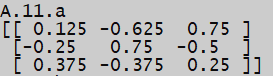
\includegraphics[width=110mm]{A11a.PNG}
\end{figure}

\subsection*{b.}

\begin{figure}[ht!]
  \centering
  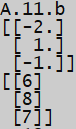
\includegraphics[width=30mm]{A11b.PNG}
\end{figure}

}

\section*{A.12}
{\Large 

Two random variables $X$ and $Y$ have equal
  distributions if their CDFs, $F_X$ and $F_Y$, respectively, are
  equal, i.e. for all $x$, $ |F_X(x) - F_Y(x)| = 0$. 
The central limit theorem says that the sum of $k$ independent,
zero-mean, variance-$1/k$ random variables converges to a (standard) Normal distribution as $k$ goes off to infinity.  
We will study this phenomenon empirically (you will use the Python packages Numpy and Matplotlib). 
Define $Y^{(k)} = \frac{1}{\sqrt{k}} \sum_{i=1}^k B_i$ where each $B_i$ is equal to $-1$ and $1$ with equal probability.
From your solution to problem 5, we know that $\frac{1}{\sqrt{k}} B_i$ is zero-mean and has variance $1/k$.

\subsection*{a.}
We found in A.6 that for all $x \in \R$, we have  $\displaystyle \E[ ( \widehat{F}_n(x) - F(x) )^2 ] \leq \tfrac{1}{4n}$. Since we aim to have $n$ large enough such that $ \sqrt{\E[(\widehat{F}_n(x)-F(x))^2 ]} \leq 0.0025$, we can take \\
$\E[ ( \widehat{F}_n(x) - F(x) )^2 ] \leq \tfrac{1}{4n}$ \\
$\sqrt{\E[ ( \widehat{F}_n(x) - F(x) )^2 ]} \leq \tfrac{1}{2\sqrt{n}}$ \\
Solving for $\frac{1}{2\sqrt{n}} = 0.0025$: \\
$400 = 2\sqrt{n}$ \\
$200 = \sqrt{n}$ \\
$n = 40,000$ \\

\begin{verbatim}
def plot_rvs(n):
  print("A.12.a")
  Z = np.random.randn(n)
  plt.step(sorted(Z), np.arange(1, n+1) / float(n), label = "Gaussian")

  plt.xlim(-3, 3)
  plt.xlabel("Observations")
  plt.ylabel("Probability")
  plt.legend()
  plt.title("A.12.a")
  plt.savefig("A12a.png")
\end{verbatim}

\begin{figure}[ht!]
  \centering
  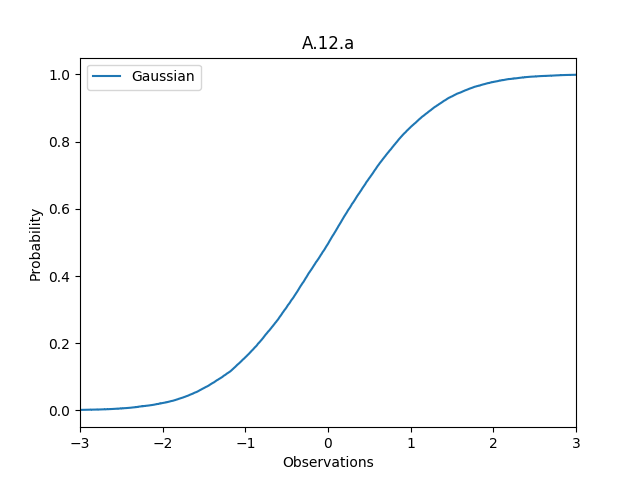
\includegraphics[width=130mm]{A12a.PNG}
\end{figure}

\subsection*{b.}
\begin{verbatim}
def generate_copies(n):
  print("A.12.b")
  k_set = [1, 8, 64, 512]

  for k in k_set:
    obs_set = np.sum(np.sign(np.random.randn(n, k)) * np.sqrt(1./k), axis=1)
    plt.plot(sorted(obs_set), np.arange(1, n+1) / float(n), label = str(k))

  plt.legend()
  plt.title("A.12.b")
  plt.savefig("A12b.png")
  plt.close()
\end{verbatim}

\begin{figure}[ht!]
  \centering
  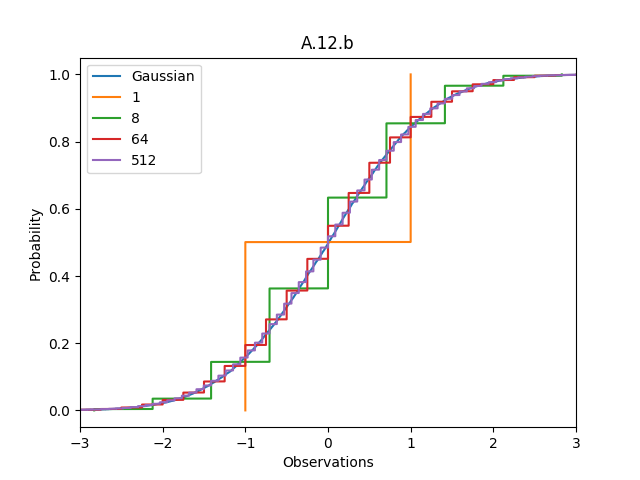
\includegraphics[width=130mm]{A12b.PNG}
\end{figure}

}

\end{document}